\documentclass[12pt]{article}
\usepackage{tikz}
\usepackage{pgfplots}
\pgfplotsset{compat=1.13}

\usepackage{extsizes}
\usepackage{caption}
\usepackage{multirow}
\usepackage{wrapfig}

\renewcommand{\epsilon}{\ensuremath{\varepsilon}}
\renewcommand{\phi}{\ensuremath{\varphi}}
\renewcommand{\kappa}{\ensuremath{\varkappa}}
\renewcommand{\le}{\ensuremath{\leqslant}}
\renewcommand{\leq}{\ensuremath{\leqslant}}
\renewcommand{\ge}{\ensuremath{\geqslant}}
\renewcommand{\geq}{\ensuremath{\geqslant}}
\renewcommand{\emptyset}{\varnothing}

\usepackage{geometry} % Простой способ задавать поля
\geometry{top=30mm}
\geometry{bottom=30mm}
\geometry{left=25mm}
\geometry{right=20mm}

\usepackage[T2A]{fontenc}			% кодировка
\usepackage[utf8]{inputenc}	
\usepackage[english,russian]{babel}   %% загружает пакет многоязыковой вёрстки
\usepackage{indentfirst}
\usepackage{subfigure}
\usepackage{amsmath,amsfonts,amssymb,amsthm,mathtools} 
\usepackage{graphicx}
\begin{document}
	\begin{minipage}{0.45\linewidth}
	Работу выполнили\\
	Юрченко Петр, 676 гр.\\
	Самохин Валентин, 676 гр.\\[2mm]
	под руководством\\
	Нухова А.\,К\,.
	\end{minipage}
	\hfill
	\begin{minipage}{0.45\linewidth}\flushright
		Маршрут~VIII \ №~2\\[3mm]
		13~февраля 2018~г.,\\
		\end{minipage}
		
		\vspace{8mm}
		\begin{center}
			\textbf{\Large Лабораторная работа №~4.3.3:}\\[\parskip]
			\LARGE Исследование разрешающей способности микроскопа методом Аббе
			\end{center}
			\vspace{0mm}
			
			\begin{center}
				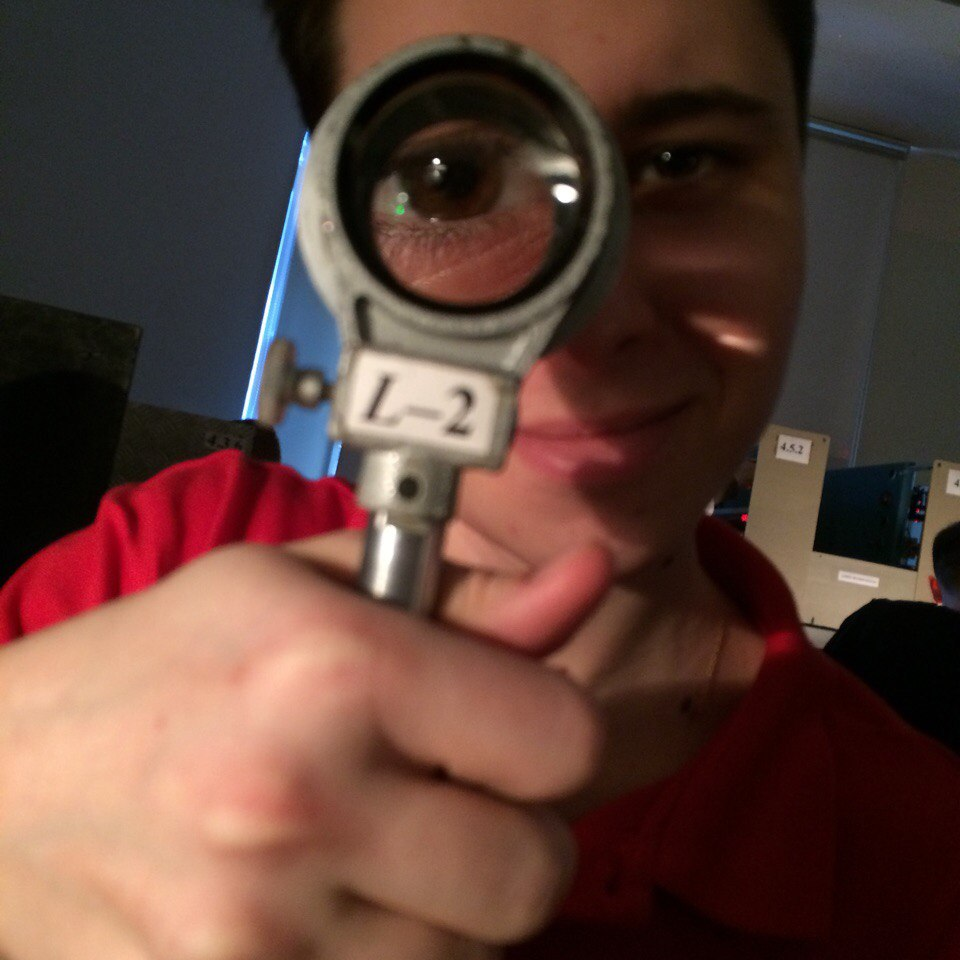
\includegraphics[scale = 0.4]{petrovich}
			\end{center}
		\thispagestyle{empty}
		\newpage
			\paragraph{Цель работы:}
			\begin{itemize}
				\item определение дифракционного предела разрешения объектива микроскопа методом Аббе
			\end{itemize}
			
			\paragraph{В работе используются:}
			лазер; кассета с набором сеток разного периода; линзы; щель с микрометрическим винтом; оптический стол с набором рейтеров и крепежных винтов; экран; линейка.
			
			
			\vspace{2\parskip}
		\paragraph{Теоретическая справка.}
		
		Всякая оптическая система, предназначенная для получения изображений, имеет конечный \textit{предел разрешения}, т. е. ограниченную возможность раздельного наблюдения близких частей предмета.
		Принципиальной причиной, ограничивающей предел разрешения, является дифракция световых волн: ограничение пучка лучей краями линз и диафрагм, составляющих оптическую систему, приводит к нарушению \textit{стигматичности изображения}\footnote{Стигматичное изображение - такое оптическое изображение, каждая точка которого соответствует одной точке изображаемого оптической системой объекта.} — каждая точка предмета отображается не в одну точку, а в дифракционное пятно.
		
		Стоит отметить, что \textit{условие применимости геометрической оптики} определяется соотношением
		\begin{equation}\label{geom_opt}
		\dfrac{\sqrt{\lambda z}}{b} \ll 1,
		\end{equation}
		
		что получается из разности фазовых набегов. При выполнении этого условия фазовые отношения между плоскими волнами, образующими поле, практически одинаковы.
		
		
		Дифракционные пятна\footnote{Дифракцией света называется явление отклонения света от прямолинейного направления распространения при прохождении вблизи препятствий. Пятно - искаженное из-за дифракции изображение.} от близких точек предмета могут перекрываться друг другом, в результате чего точки становятся неразличимыми.
		
		\textit{Разрешающей способностью оптического прибора} называют минимальное расстояние $l_{min}$ между двумя точками в пространстве предметов, изображения которых разрешаются по критерию Релея.
		
		Согласно качественному критерию, предложенному \textit{Рэлеем}, два источника света различимы, если дифракционный максимум одного источника приходится на минимум другого, иными словами расстояние между центрами пятен $\Delta x$ равно полуширине \textit{пятна Эйри}\footnote{Пятно Эйри - центрально яркое дифракционное пятно, в котором концентрируется подавляющая доля светового потока}.
		\begin{equation}\label{eq::reley}
		\Delta x = \xi_0 = 1,22\frac{\lambda}{D}z_2
		\end{equation}
		Смещению пятен $\Delta x$ в плоскости изображения соответствует расстояние между точечными источниками во входной плоскости (на расстоянии $z_1$ от линзы), равное $l =\frac{z_1}{z_2}\Delta x$. Мы получаем оценку минимального разрешимого расстояния между точечными источниками:
		\begin{equation}\label{eq::min_l}
		l_{min} \simeq 1,22\dfrac{\lambda}{D}z_1
		\end{equation}
		
		Если рассматриваются удалённые объекты, то обычно говорят об угловом разрешении $\alpha = \frac{l}{z_1}$. Изображение оказывается при этом в фокальной плоскости линзы (при $z_1 \rightarrow \infty$, $z_2 \rightarrow f$). Согласно \eqref{eq::reley}, имеем
		
		\begin{equation}
			\alpha_{min} \simeq 1,22 \dfrac{\lambda}{D}.
		\end{equation}
		
		Для \textit{иммерсионного микроскопа} (объект находится в иммерсионной среде — жидкости с показателем преломления $n$) разрешающая способность объектива
		\begin{equation}
		l_{min} \simeq \dfrac{0,61\lambda}{n\sin u} \simeq \dfrac{\lambda}{2n\sin u},
		\end{equation}
		
		где $u$ - апертурный\footnote{Апертурный - угол между оптической осью и лучом, направленным из центра объекта в край линзы} угол объектива микроскопа (рис. \ref{fig::creation_of_image}).
		\begin{figure}
			\centering
			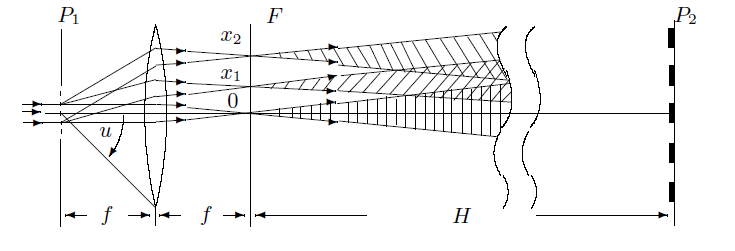
\includegraphics{1}
			\caption{Образование изображения в объективе микроскопа.
				$P_1$ — плоскость предмета, $F$ - задняя фокальная плоскость объектива,
				$P_2$ — плоскость, сопряженная с предметной плоскостью.
				В плоскости $P_2$ световые пучки сильно
				перекрываются}
			\label{fig::creation_of_image}
		\end{figure}
	
	Если наблюдения с помощью микроскопа ведутся при внешнем освещении, то,
	как правило, различные точки предмета рассеивают
	когерентные волны. Теория разрешающей способности для случая освещаемых 
	объектов была разработана Аббе.
	
	Для простоты рассмотрим случай, когда предметом является периодическая структура (дифракционная решетка), освещаемая	параллельным пучком лучей.
	
	Аббе предложил рассматривать прохождение лучей от предмета к изображению в два этапа.
	Сначала рассматривается
	картина, возникающая в задней фокальной плоскости
	$F$ объектива. Эта
	картина называется \textit{первичным изображением} или \textit{фурье-образом} предмета. Затем первичное изображение	рассматривается	как источник волн, создающих изображение предмета в плоскости
	$P_2$, сопряженной плоскости предмета, т. е. \textit{вторичное изображение}. Такой подход основан на \textit{принципе Гюйгенса–Френеля}\footnote{Согласно
	принципу Гюйгенса-Френеля любой участок волнового фронта можно рассматривать как вторичный источник излучения.}

	Первичное изображение, наблюдаемое в задней фокальной плоскости объектива, представляет собой картину дифракции Фраунгофера на объекте (в нашем случае
	— на дифракционной решет-
	ке). Действительно, на решетку падает плоская волна, а каждая точка	наблюдения в фокальной плоскости $F$ линзы соответствует бесконечно удаленной точке. Смещение $x_m$ точки наблюдения от оптической оси связано с углом наклона $\varphi_m$ параллельного пучка лучей перед линзой соотношением (при малых $\varphi$): $x_m \simeq f\varphi_m$.
	\begin{figure}
		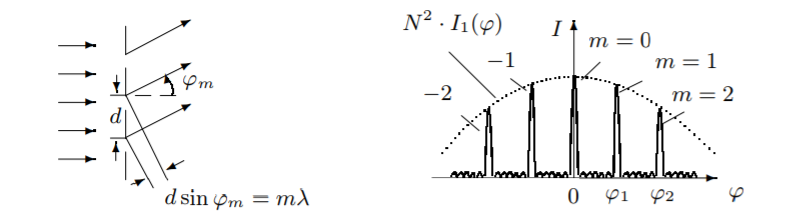
\includegraphics{2}
		\caption{Спектр амплитудной решетки. $I_1(\varphi)$ — распределение интенсивности
			при дифракции света на одиночной щели.}
		\label{fig::difrac}
	\end{figure}

	При дифракции Фраунгофера на одномерной решетке периода	$d$ направления $\varphi_m$ максимальной интенсивности (главные максимумы) определяются
	условием:
	\begin{equation}
	d\sin\varphi_m = m\lambda,
	\label{eq::main_max}
	\end{equation}
	
	Первичное изображение представляет собой набор ярких точек, расположенных цепочкой на равных расстояниях друг от друга. Излучение	этих когерентных точечных источников создаст в плоскости	$P_2$ систему
	интерференционных полос, синтезирующих изображение предмета (решетки) в этой плоскости.
	
	В силу конечного диаметра линзы, часть первичного изображения закрывается, через микроскоп проходят только те пучки, для которых выполняется условие $\varphi_m < u$.
	Эти пучки лучей собираются в задней фокальной плоскости линзы, так что за ней возникают рас
	ходящиеся пучки лучей с центрами в плоскости $F$. В плоскости $P_2$ эти пучки
	интерферируют и воспроизводят увеличенное изображение решетки.
	
	Диафрагмы практически одинаковых размеров, расположенные в фокальной плоскости
	$F$ или непосредственно на объективе, перекрывают те же самые пучки лучей.
	Таким образом, дифракцию на оправе объектива в рассмотрении Аббе можно заменить дифрак-
	цией на диафрагме $D$, равной по размеру диаметру работающей (открытой) части линзы
	и расположенной в задней фокальной плоскости
	$F$.
	
	Если приоткрыть диафрагму и поставить ее несимметрично, так, чтобы прошел только нулевой и один из первых максимумов, то на экране
	получится изображение, имеющее вид периодической структуры с плавным переходом от светлых мест к темным; такое изображение характерно для двухлучевой интерференции.
	Рассчитаем период изображения в
	плоскости $P_2$ для этого случая. Линейное расстояние
	$x_1$ между максимумами нулевого
	и первого порядка в плоскости $F$ есть
	$$x_1 \simeq f\varphi_1 = f\lambda/d$$
	
	Ширина $l$ интерференционных полос, образующихся в плоскости $P_2$, может быть найдена по формуле
	$$ l = \lambda/\omega$$
	где $\omega	= x_1/H$
	— угол схождения интерферирующих лучей в точке наблюдения, расположенной в плоскости
	$P_2$, а $H$
	— расстояние между плоскостями
	$F$ и $P_2$. Таким образом,
	$$l \simeq \lambda H/x_1 = Hd/f$$
	
	Согласно геометрической оптике изображение решетки в плоскости
	$P_2$ должно иметь период
	$$d' \simeq \dfrac{H+f}{f}d$$
	В силу того, что $H >> f$, $l \simeq d'$.
	Таким образом, с помощью дифракционных максимумов нулевого
	и первого порядка в увеличенном масштабе передается основной
	период решетки (и не воспроизводятся никакие детали структуры).

	
	Если задержать каким-либо образом в плоскости
	$F$ максимум первого порядка, а вместо него пропустить максимум второго порядка, то
	в $P_2$ возникнет система полос с периодом в два раза меньшим, так что на экране будет видно изображение более частой решетки, чем имеющаяся в действительности. Максимумы высших порядков создают более узкие интерференционные полосы, они ответственны за передачу более
	тонких деталей. Из изложенного ясно, что для получения правильного изображения
	надо, чтобы через объектив микроскопа про
	ходили дифракционные пучки разных направлений. Как уже отмечалось ранее, если апертурный
	угол $u$ меньше
	$\varphi_1$, то в плоскости
	$P_2$ не возникает периодического изображения. Соотношение $\sin u \geqslant \lambda/d$ можно рассматривать	как
	условие разрешения решетки с периодом
	$d$.
	Отсюда можно найти минимальное разрешаемое объективом расстояние
	\begin{equation}\label{eq::min_dist}
	d \geq \dfrac{\lambda}{\sin u} \simeq \dfrac{\lambda}{(D/2f)}
	\end{equation}
	При этом диафрагма $D$, расположенная симметрично, пропускает нулевой и
	$\pm$1 максимумы.
	
	При освещении решётки пучками, наклонными
	к оси,
	когда через
	диафрагму, кроме нулевого, про
	ходит всего один из двух первых максимумов (этого достаточно для изображения периодической структуры
	без тонких деталей),
	условие разрешения принимает вид
	$$d \geq \dfrac{\lambda}{2\sin u}$$
	
	В нашей работе применяется двумерная решетка
	— сетка. Ее можно рассматривать
	как две скрещенные (перпендикулярные друг к другу) решетки.
	Главные максимумы возникают тогда,
	когда одновременно выполняются
	условия:
	$$d\sin \varphi_x = m_x\lambda, \; \; d\sin \varphi_y = m_y\lambda.$$
	
	Максимумы, удовлетворяющие
	условию $\varphi_x, \varphi_y <
	u$, создают в задней
	фокальной плоскости
	$F$ объектива
	картину дифракции Фраунгофера (рис. \ref{fig::frau}) 
	— первичное изображение.
	
	\begin{wrapfigure}{r}{.4\textwidth}
		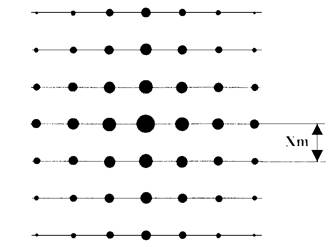
\includegraphics{3}
		\caption{Дифракция Фраунгофера на двумерной решетке
			(сетке). Максимумы изображены кружками, размеры которых характеризуют интенсивности}
		\label{fig::frau}
	\end{wrapfigure}

	Если теперь поместить в фокальной плоскости вертикальную щель так, чтобы
	через нее проходили дифракционные максимумы с $m_x = 0$ и
	$m_y = 0, \pm 1, \pm 2, \dots$,
	то в плоскости
	$P_2$ получится изображение
	решетки с горизонтально расположенными штрихами. Если, наоборот, пропустить
	максимумы с $m_y = 0$ и
	$m_x = 0, \pm1, \pm2, \dots$,
	то в $P_2$ получится изображение решетки
	с вертикальными штрихами.
	Таким образом можно продемонстрировать явление
	\textit{пространственной фильтрации}
	— выделение различных структур в изображении.
	
	\paragraph{Экспериментальная установка}
	Схема модели проекционного микроскопа приведена на рис. \ref{fig::exp}. Предметом служат сетки, расположенные в кассете. Смена сеток осуществляется поворотом внешнего кольца кассеты.

	Излучение лазера (ОКГ) почти перпендикулярно падает на сетку С,
	установленную вблизи фокальной плоскости линзы
	Л$_1$ — объектива микроскопа. Вторичное изображение из плоскости
	$P_2$ проецируется на экран Э линзой
	Л$_2$ (короткофокусной, чтобы изображение на экране
	было крупнее). 
	
	Изображение сетки периодически повторяется — \textit{репродуцируется} —
	в пространстве между сеткой и первой линзой, поэтому для того, чтобы среди множества репродуцированных изображений
	сетки можно было выделить её геометрическое изображение, на одну из
	сеток нало
	жена тонкая проволочка, т.е. непериодический объект, изображение
	которого не репродуцируется.
	
	В фокальной плоскости $F$ могут быть
	установлены диафрагмы — щелевая или ирисовая (отверстие с переменным диаметром)
	и различного рода маски (препятствия).
	
	Имея набор сеток с
	различными периодами
	$d$
	и изменяя апертурный угол объектива с помощью щелевой диафрагмы, можно экспериментально проверить соотношение \eqref{eq::min_dist}.
	
	В нашей работе период сеток рассчитывается двумя способами: в первом способе (дифракция Фраунгофера) — расстояние между дифракционными максимумами на экране измеряется при помощи линейки, а затем по формуле решетки \eqref{eq::main_max} определяется ее период; во втором способе
	период определяется по увеличенному с помощью модели микроскопа
	изображению сетки на экране.
	
	С помощью откалиброванных таким образом сеток определяется разрешающая способность микроскопа. Для этого в задней фокальной плоскости
	$F$ объектива устанавливается щелевая диафрагма с микрометрическим винтом
	и подбирается ее минимальный размер, при
	котором еще	видно изображение сетки на экране (щель пропускает максимумы с $m =
	= 0, \pm1$). По размеру диафрагмы
	и фокусному расстоянию объектива
	рассчитывается апертурный угол
	$u$
	и проверяется соотношение \eqref{eq::min_dist}.
	
	
	Для выполнения последней части работы ширина вспомогательной
	щели
	и угол наклона
	к оси системы подбираются так, чтобы на экране
	вместо изображения сетки получалось изображение решётки, расположенной наклонно, т. е. осуществлялась \textit{пространственная фильтрация}.
	Если сетку
	и щель поменять местами, то соответствующим подбором сетки можно «рассечь» первичное изображение так, что изображение щели
	на экране будет многократно повторяться
	— \textit{мультиплицироваться}.
	\begin{figure}
		\centering
		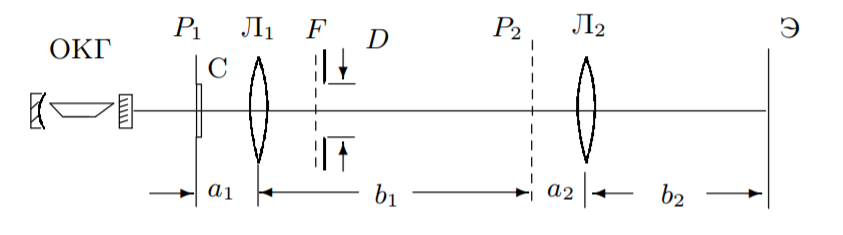
\includegraphics{4}
		\caption{Схема экспериментальной установки - модель проекционного микроскопа}
		\label{fig::exp}
	\end{figure}

	\paragraph{Обработка результатов}
	\subparagraph{Определение периода решёток по их пространственному спектру}
	Сначала мы определяли расстояние между соседними дифракционными максимумами. Для увеличения точности мы замеряли расстояние между удаленными друг от друга максимумами и число промежутков между ними.
	\begin{center}
	\begin{tabular}{|c|c|c|c||c|c|}
		\hline
		\multicolumn{6}{|c|}{Решетка №1} \\
		\hline 
		\multicolumn{2}{|c|}{Горизонталь}& \multicolumn{2}{|c||}{Вертикаль} & $\overline{\Delta_{x}}$, мм & $35,0\pm 0,5$ \\ 
		\hline 
		$l$, мм  & $n$ & $l$, мм & $n$ & $\overline{\Delta_{y}}$, мм & $34,9 \pm 0,1$\\ 
		\hline 
		243 & 7 & 209 & 6 & $\theta_x$ & $0,026 \pm 0,003$\\ 
		\hline 
		174 & 5 & 173 & 5 & $\theta_y$ & $0, 026 \pm 0,001$\\ 
		\hline 
		104 & 3 & 140 & 4 &$d_x$, мм & $0,021 \pm 0,001$ \\ 
		\hline 
		36 & 1 & 105 & 3 & $d_y$, мм & $0,0206 \pm 0,0002$\\ 
		\hline
		\multicolumn{6}{|c|}{Решетка №2} \\
		\hline 
		\multicolumn{2}{|c|}{Горизонталь}& \multicolumn{2}{|c||}{Вертикаль}  & $\overline{\Delta_{x}}$, мм & $23,20 \pm 0,03$\\ 
		\hline 
		$l$, мм  & $n$ & $l$, мм & $n$  & $\overline{\Delta_{y}}$, мм & $23,19 \pm 0,04$\\ 
		\hline 
		232 & 10 & 186 & 8 & $\theta_x$ & $0,0172\pm 0,0002$  \\ 
		\hline 
		209 & 9 & 162 & 7 & $\theta_y$ & $0,0171 \pm 0,0003$\\ 
		\hline 
		186 & 8 & 139 & 6 & $d_x$, мм& $0,0310 \pm 0,0002$ \\ 
		\hline 
		162 & 7 & 116 & 5 & $d_y$, мм& $0,0310 \pm 0,0001$ \\ 
		\hline
		\multicolumn{6}{|c|}{Решетка №3} \\
		\hline 
		\multicolumn{2}{|c|}{Горизонталь}& \multicolumn{2}{|c||}{Вертикаль}  & $\overline{\Delta_{x}}$, мм & $11,59 \pm 0,02$\\ 
		\hline 
		$l$, мм  & $n$ & $l$, мм & $n$  & $\overline{\Delta_{y}}$, мм & $11,56 \pm 0,03$\\ 
		\hline 
		197 & 17 & 139 & 12 & $\theta_x, 10^{-3}$ & $8,6 \pm 0,1$ \\ 
		\hline 
		185 & 16 & 127 & 11 & $\theta_y, 10^{-3}$ & $8,6 \pm 0,3$\\ 
		\hline 
		174 & 15 & 115 & 10 & $d_x$, мм  & $0,0620 \pm 0,0002$\\ 
		\hline 
		162 & 14 & 104 & 9 & $d_y$, мм & $0,0621 \pm 0,001$\\ 
		\hline
		\multicolumn{6}{|c|}{Решетка №4} \\
		\hline
		\multicolumn{2}{|c|}{Горизонталь}& \multicolumn{2}{|c||}{Вертикаль}  & $\overline{\Delta_{x}}$, мм & $5,76 \pm 0,01$ \\ 
		\hline 
		$l$, мм  & $n$ & $l$, мм & $n$  & $\overline{\Delta_{y}}$, мм & $6,1 \pm 0,1$ \\ 
		\hline 
		138 & 24 & 110 & 18 & $\theta_x, 10^{-3}$ & $4,3 \pm 0,1$\\ 
		\hline 
		127 & 22 & 16 & 98 & $\theta_y, 10^{-3}$ & $4,6 \pm 0,4$\\ 
		\hline 
		115 & 20 & 14 & 87 & $d_x$, мм & $0,125 \pm 0,001$\\ 
		\hline 
		104 & 18 & 12 & 75 & $d_y$, мм & $0,12 \pm 0,03$\\ 
		\hline
		\multicolumn{6}{|c|}{Решетка №5} \\
		\hline
		\multicolumn{2}{|c|}{Горизонталь}& \multicolumn{2}{|c||}{Вертикаль}   & $\overline{\Delta_{x}}$, мм & $4,5$ \\
		\hline 
		$l$, мм  & $n$ & $l$, мм & $n$ & $\overline{\Delta_{y}}$ & $4,53 \pm 0,03$\\ 
		\hline 
		117 & 26 & 99 & 22 & $\theta_x, 10^{-3}$ & $3,3$\\ 
		\hline 
		108 & 24 & 90 & 20 & $\theta_y, 10^{-3}$ & $3,4 \pm 0,2$\\ 
		\hline 
		99 & 22 & 82 & 18 & $d_x$, мм & $0,16$ \\ 
		\hline 
		90 & 20 & 73 & 16 & $d_y$ & $0,16 \pm 0,03$\\ 
		\hline 
	\end{tabular} 
	\captionof{table}{Данные для подсчета периода решетки}
	\end{center}
	
	
	По полученным данным подсчитали дифракционные углы и периоды решеток.
	
	\paragraph{Определение периода решёток по изображению, увеличенному	с помощью модели микроскопа}
	Собрав модель микроскопа и определив его увеличение, найдем период решетки по периоду его изображения.
	
	Запишем параметры установки и найдем увеличение системы (см. рис. \ref{fig::exp}).
	
	\begin{minipage}{.48\textwidth}
		$a_1 = 51$ мм\\
		$a_2 = 80$ мм\\
		$b_1 = 350$ мм\\
		$b_2 = 685$ мм\\
	\end{minipage}
	\hfill
	\begin{minipage}{.48\textwidth}
		$\Gamma = \dfrac{b_1b_2}{a_1a_2}$ \\
		\fbox{$\Gamma = 58,8 \pm 1,5$}
	\end{minipage}
	
	\begin{center}
	\begin{tabular}{|c|c||c|c||c|c||c|c|}
		\hline
		\multicolumn{2}{|c||}{Решетка №5} & \multicolumn{2}{|c||}{Решетка №4} & \multicolumn{2}{|c||}{Решетка №3} & \multicolumn{2}{|c|}{Решетка №2} \\
		\hline 
		$n$ & $l$, мм & $n$ & $l$, мм & $n$ & $l$, мм & $n$ & $l$, мм \\ 
		\hline 
		1 & 9 & 1 & 7 & 1 & 4 & 5 & 9 \\ 
		\hline 
		2 & 18 & 2 & 14 & 2 & 7 & 7 & 12,5 \\ 
		\hline 
		3 & 27 & 3 & 20 & 3 & 10 &  &  \\ 
		\hline 
		$d$ & $0,153\pm 0,004$ & $d$ & $0,117 \pm 0,003$ & $d$ & $0,060\pm 0,002$ & $d$ & $0,0305\pm 0,001$ \\ 
		\hline 
		$d_I$ & $0,16 \pm 0,03$ & $d_I$ & $0,125 \pm 0,03$ & $d_I$ & $0,0621 \pm 0,001$ & $d_I$ & $0,0310 \pm 0,0001$  \\ 
		\hline 
	\end{tabular} 
	\captionof{figure}{Данные для определения периода решеток по изображению}
		\end{center}
	
	\paragraph{Определение периодов решёток по оценке разрешающей способности
		микроскопа}
	
	Для каждой решетки запишем минимальный размер диафрагмы, при котором еще видно \underline{сетку}.
	По формуле $\eqref{eq::min_dist}$ определим период решетки.
	\begin{center}
	\begin{tabular}{|c|c|c|c|c|}
		\hline 
		$n$ решетки & 2 & 3 & 4 & 5 \\ 
		\hline 
		D, мм & 3,53 & 1,63 & 1 & 0,76 \\ 
		\hline
		$d$, мм & $0,033 \pm 0,001$ & $0,072 \pm 0,001$&$0,117 \pm 0,001$ &$0,154 \pm 0,001$ \\
		\hline 
	\end{tabular}
	\captionof{table}{Вычисления по ширине щели} 
	\end{center}
	
	\paragraph{Проверка теории Аббе}
	Для проверки теории Аббе построим график зависимости $d = f(1/D)$ (рис.\ref{fig::graph}),
	взяв периоды сеток, определённые по \underline{спектру}. Проверим справделивость формулы \eqref{eq::min_dist}.
	
	\begin{center}
		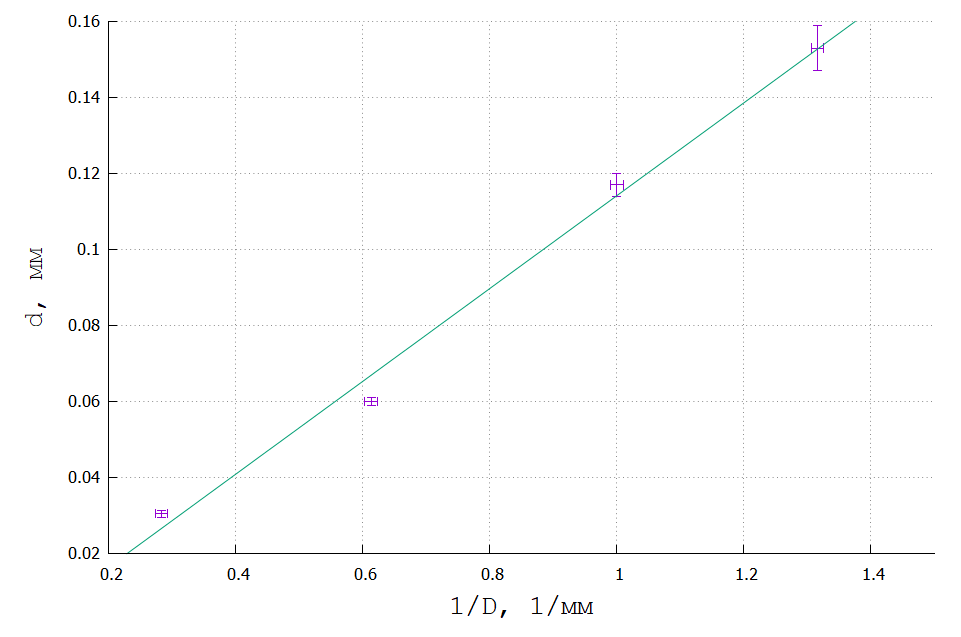
\includegraphics[scale= 0.8]{graph}
		\captionof{figure}{График зависимости $d = f(1/D)$}
		\label{fig::graph}
	\end{center}	
	
		
	\paragraph{Наблюдение пространственной фильтрации и мультиплицирования}
	\subparagraph{Пространственная фильтрация}
	Ширину щели подберем так, чтобы она свободно пропускала максимум нулевого порядка и не пропускала максимумы первого порядка, расположенные в поперечном направлении. Поворачивая щель
	относительно оси системы, получим изображения решёток при различных ориентациях щели (рис. \ref{fig:filter}). При наклоне под углом $45^{\circ}$ на экране видна наклонная решётка - периодическая структура, которой нет в исходном объекте.
	
	\begin{figure}  
		\vspace{-4ex} \centering \subfigure[]{
			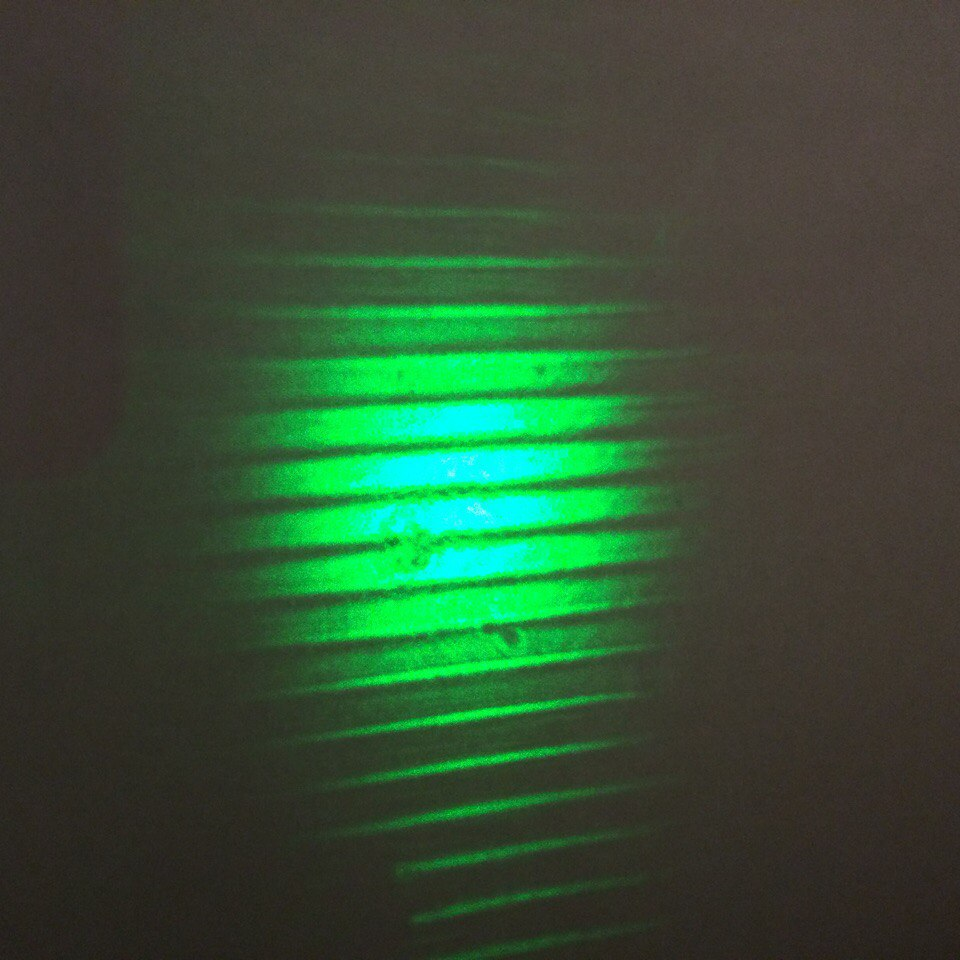
\includegraphics[width=0.25\linewidth]{parallels}\label{fig::parallels} }  
		\hspace{4ex}
		\subfigure[]{
			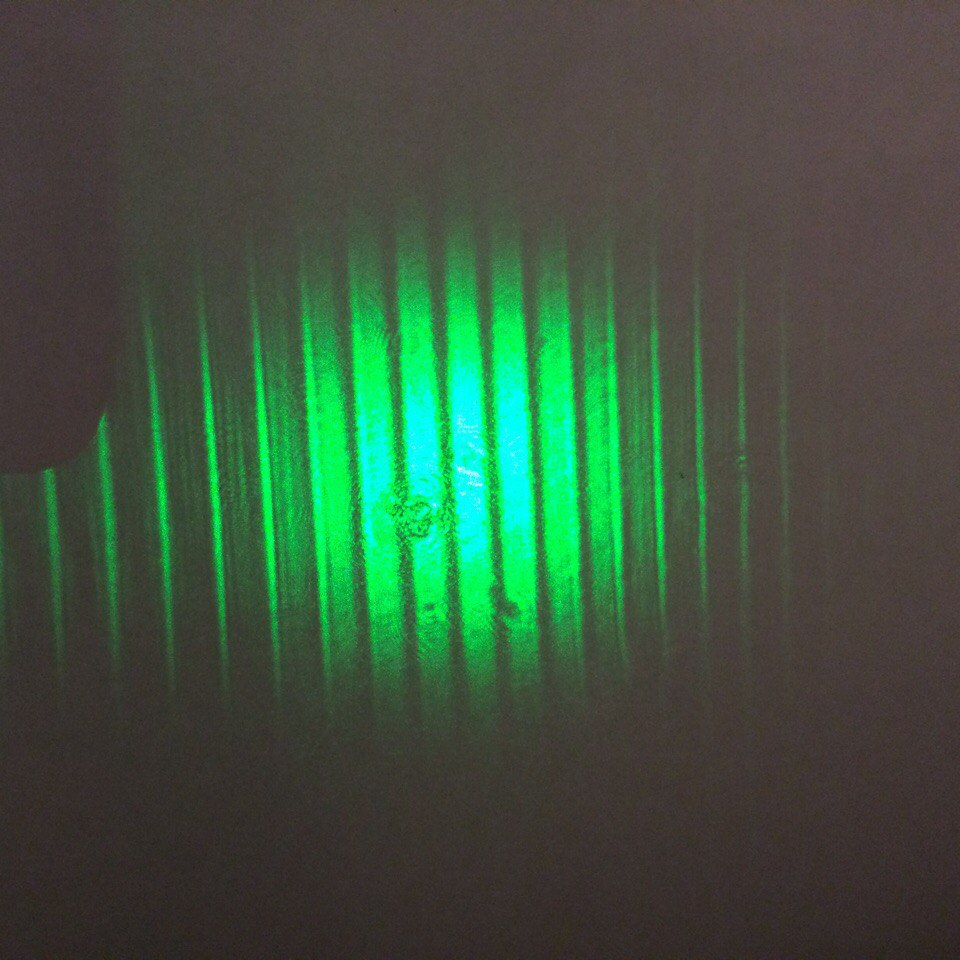
\includegraphics[width=0.25\linewidth]{vertical}\label{fig::vertical}}
		\hspace{4ex}
		\subfigure[]{ 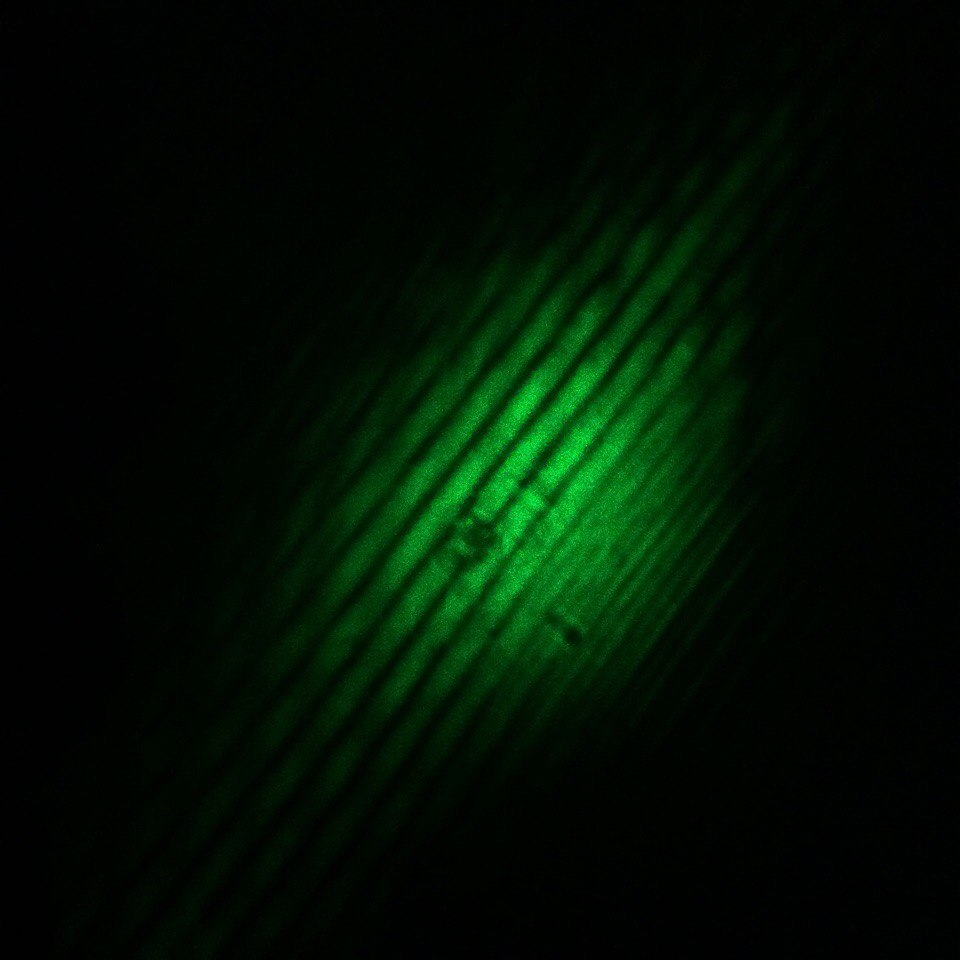
\includegraphics[width=0.25\linewidth]{forty_five}\label{fig::ff}}  
		\caption{Периодические структуры на экране: \subref{fig::parallels} при вертикальной ориентации щели; \subref{fig::vertical} при горизонтальной ориентации щели; \subref{fig::ff} при наклоне под углом в $45^{\circ}$.} \label{fig:filter}
	\end{figure}

	\subparagraph{Мультиплицирование}
	Подберем такую ширину входной щели $D$, чтобы на экране можно было наблюдать мультиплицированное изображение (рис. \ref{fig:multi}) для всех сеток.	Чем уже щель, тем шире её фурье-образ и тем легче рассечь его
	сетками.
	
	\begin{figure} 
		\vspace{-4ex} \centering \subfigure[]{
			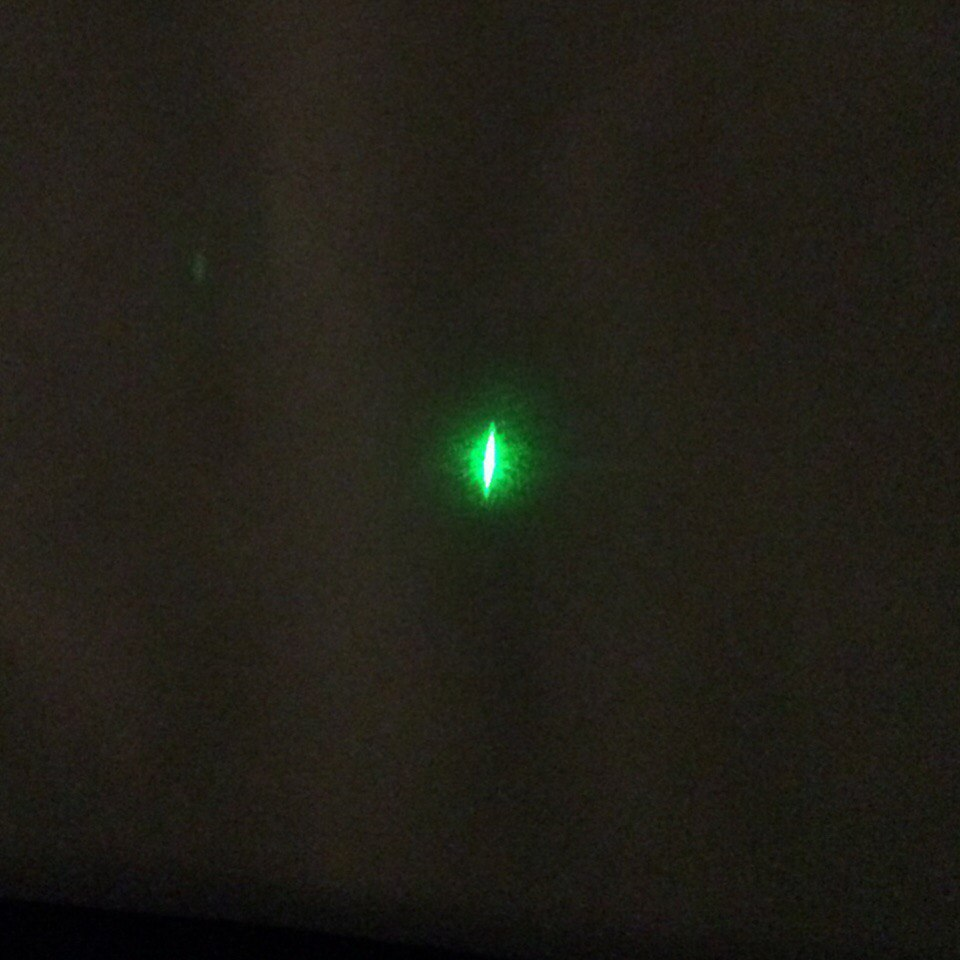
\includegraphics[width=0.25\linewidth]{single_hole}\label{fig::single} }  
		\hspace{4ex}
		\subfigure[]{
			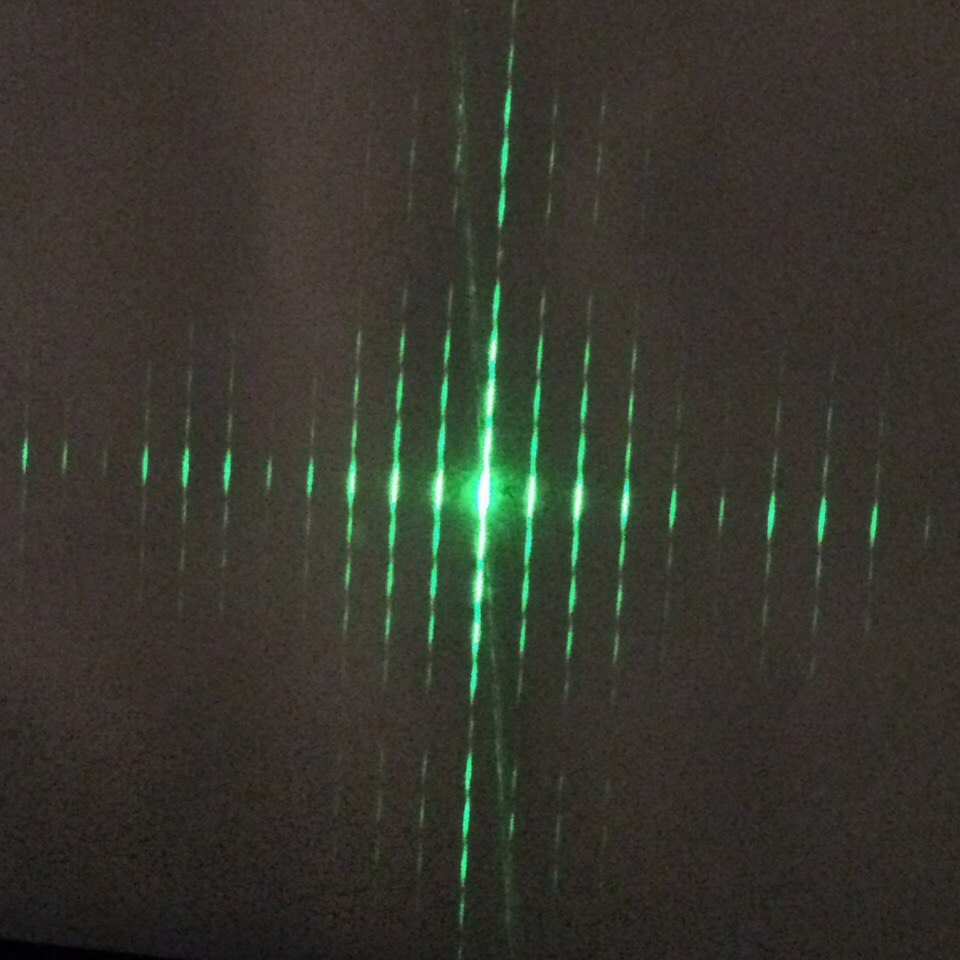
\includegraphics[width=0.25\linewidth]{many_holes}\label{fig::many}}
		\hspace{4ex}
		\subfigure[]{ 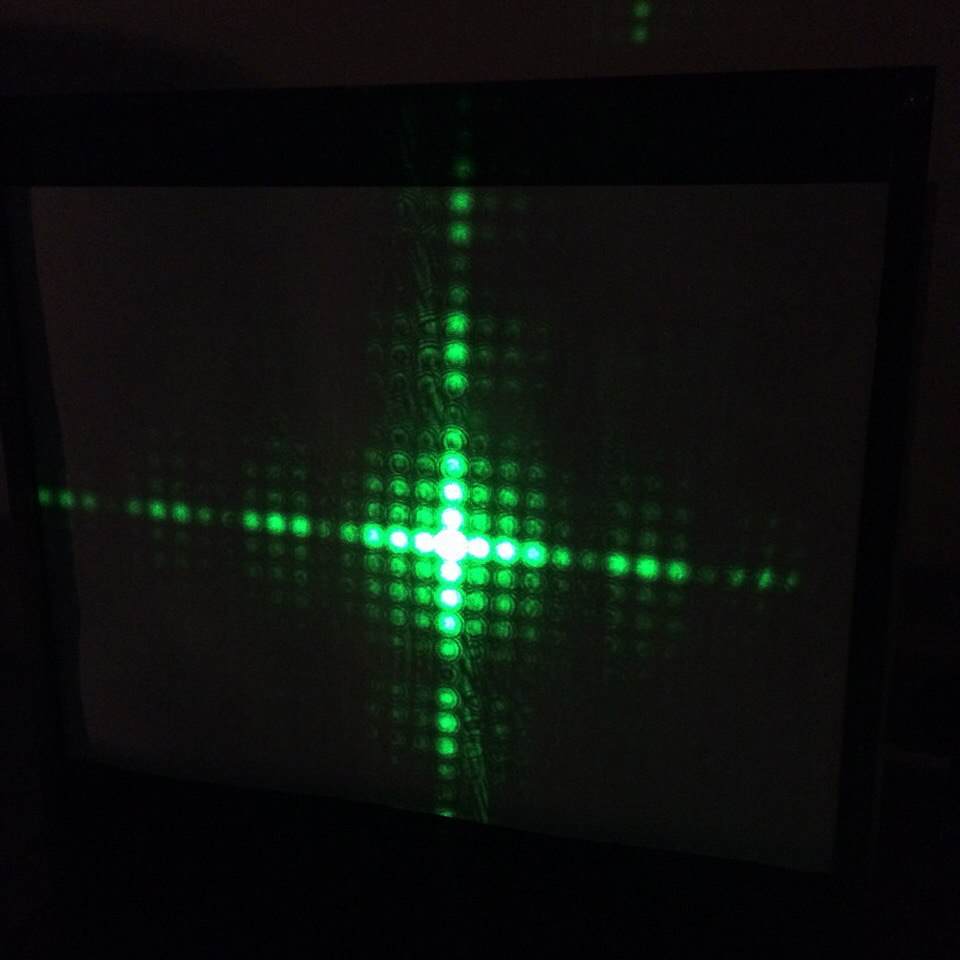
\includegraphics[width=0.25\linewidth]{wide_hole}\label{fig::wide}}  
		\caption{Наблюдение мультиплицирования: \subref{fig::single} четкое изображение щели; \subref{fig::many} ширина щели меньше; \subref{fig::wide} ширина щели больше.} \label{fig:multi}
	\end{figure}
	
	\paragraph{Вывод}
	В данной лабораторной работе мы познакомились с дифракцией, собрали модель микроскопа и попытались найти его разрешающую способность. С основной задачей - найти период изображения (сетки) - мы справились, однако всилу миниатюрных размеров не только объекта, но и изображения, мы столкнулись с ошибкой, в следствие чего результаты некоторых экспериментов незначительно расходились. Кроме того, на основе полученных данных, мы смогли убедиться в справедливости теории Аббе, а также формулы \eqref{eq::min_dist}, дающей информацию об минимальной апертуре микроскопа.
	\end{document}		
